\documentclass[11pt]{article}
\usepackage[margin=1in]{geometry}
\usepackage{volfit_preamble}
\graphicspath{{figures/}}

\title{\textbf{From Ranks to Smiles}\\[2pt]
\large LQD as a monotone transport and pricing engine\\[2pt]
\normalsize Vol-Fitter Technical Notes, No.~01}
\author{Vol-Fitter}
\date{\today}

\begin{document}
\maketitle

% Auto-generated by Docs/notes/figures/gen_lqd_fresh.py -- do not edit.
% Exact-20%-ATM half-year logistic toy.
\newcommand{\lqdfreshtoyexpiry}{0.50}
\newcommand{\lqdfreshtoyatm}{20.0000}
\newcommand{\lqdfreshtoyscale}{0.08125025}
\newcommand{\lqdfreshtoymu}{-0.01088288}
\newcommand{\lqdfreshtoyuatm}{0.533436}
\newcommand{\lqdfreshtoyuatmpct}{53.3436}
\newcommand{\lqdfreshtoyuten}{0.796524}
\newcommand{\lqdfreshtoystriketen}{1.105171}
\newcommand{\lqdfreshtoyshareten}{0.24722094}
\newcommand{\lqdfreshtoycashten}{0.22487593}
\newcommand{\lqdfreshtoycallten}{0.02234501}
\newcommand{\lqdfreshtoycalltenpct}{2.2345}
\newcommand{\lqdfreshtoyivten}{20.5977}
% SPX-like production fit.
\newcommand{\lqdfreshspxorder}{9}
\newcommand{\lqdfreshspxnquotes}{24}
\newcommand{\lqdfreshspxatm}{21.7961}
\newcommand{\lqdfreshspxskew}{-0.177846}
\newcommand{\lqdfreshspxcurvature}{0.002673}
\newcommand{\lqdfreshspxmaxerr}{1.341}
\newcommand{\lqdfreshspxrmserr}{0.408}
\newcommand{\lqdfreshspxnfev}{8}
\newcommand{\lqdfreshspxAL}{0.157473}
\newcommand{\lqdfreshspxAR}{0.037786}
\newcommand{\lqdfreshspxbetaL}{0.073087}
\newcommand{\lqdfreshspxbetaR}{0.019259}
\newcommand{\lqdfreshspxvarswap}{22.9685}
\newcommand{\lqdfreshspxmart}{\ensuremath{-1.11\times10^{-16}}}
% Asymmetric double-hat event fit.
\newcommand{\lqdfresheventorder}{16}
\newcommand{\lqdfresheventnquotes}{37}
\newcommand{\lqdfresheventweightleft}{56.0}
\newcommand{\lqdfresheventmeanleft}{-0.074804}
\newcommand{\lqdfresheventmeanright}{0.085196}
\newcommand{\lqdfresheventmaxerr}{2.444}
\newcommand{\lqdfresheventrmserr}{0.999}
\newcommand{\lqdfresheventAL}{0.015531}
\newcommand{\lqdfresheventAR}{0.014044}
\newcommand{\lqdfresheventmart}{\ensuremath{-2.22\times10^{-16}}}
\newcommand{\lqdfresheventmaxquotediv}{2.444}
% Convexity and derivative checks.
\newcommand{\lqdfreshminbutterfly}{0.224428}
\newcommand{\lqdfreshbutterflyrelerr}{0.0182}
\newcommand{\lqdfreshjacnparams}{10}
\newcommand{\lqdfreshjacmaxrel}{\ensuremath{2.88\times10^{-5}}}
% Ready-to-drop worked-example tables.
\newcommand{\lqdfreshtoytable}{%
\begin{tabular}{lr}
\toprule
Quantity & Production value\\
\midrule
Solved scale & 0.08125025\\
Martingale shift & -0.01088288\\
ATM percentile & 53.3436\%\\
$C(0.10)$ & 0.02234501\\
$\sigma_{\mathrm{BS}}(0.10)$ & 20.5977\%\\
\bottomrule
\end{tabular}}
\newcommand{\lqdfreshfitdiagtable}{%
\begin{tabular}{lrr}
\toprule
Diagnostic & SPX-like & Event\\
\midrule
Model order & 9 & 16\\
Quotes & 24 & 37\\
Max error (vol bp) & 1.341 & 2.444\\
RMS error (vol bp) & 0.408 & 0.999\\
$A_L$ & 0.157473 & 0.015531\\
$A_R$ & 0.037786 & 0.014044\\
\bottomrule
\end{tabular}}


\begin{abstract}
For one expiry, a volatility smile is the price-screen image of a probability
law.  This note builds that law from a single logistic draw and an increasing
\emph{rubber ruler}.  The ruler says how fast successive probability ranks
travel through log-return space.  Its speed is positive by construction, a
scalar translation makes the normalized asset a martingale, and one endpoint
inequality is the exact price of having a finite forward.  From there, option
pricing becomes the difference of two tail ledgers.  The same upper-share
ledger also supplies the analytic calibration Jacobian and the natural
cross-expiry convex-order test.

This transport view is mathematically identical to the production LQD family,
but it does not use the customary log-quantile-density formula as its narrative
spine.  We derive the density, the no-butterfly result, the moment strip, Lee
wing slopes, exact ATM level/skew/curvature identities, calibration controls,
and calendar ordering from the transport itself.  The worked cases include an
exact constant-speed unit check, a production SPX-like fit with
\lqdfreshspxmaxerr\ volatility-basis-point maximum error, an event distribution
with two landing zones, and an analytic-versus-finite-difference Jacobian
audit.  The aim is a lecture that a quant can prove and a trader can use: few
symbols, explicit trade tickets, and a sharp distinction between structural
guarantees and numerical controls.
\end{abstract}

\tableofcontents
\newpage

%======================================================================
\section{One random number, one expiry}
\label{sec:one_draw}

Forget the volatility screen for a moment.  Imagine a lottery drum containing
all ranks from zero to one.  We draw one rank $p$, turn it into a real-valued
score, and then decide where that score lands on the log-return axis.  If the
landing map is increasing, ranks never cross.  That innocent observation is
the whole architectural idea behind LQD.

Fix an expiry $T$.  Let $F_T$ be its forward price and $D_T$ its discount
factor.  Expectations are under the $T$-forward pricing measure, with
deterministic proportional carry.  Normalize:
\begin{equation}
Y=\frac{S_T}{F_T},\qquad X=\log Y,\qquad
k=\log\frac{K}{F_T},\qquad \E[Y]=1 .
\label{eq:normalization}
\end{equation}
The undiscounted call in forward units is
\begin{equation}
c(k)=\frac{C^\$(F_Te^k,T)}{D_TF_T}
    =\E\!\left[(Y-e^k)^+\right].
\label{eq:normalized_call}
\end{equation}
Actual dollars return by multiplying by $D_TF_T$.  Until then, the forward is
one and the strike is $e^k$.

\subsection{The seed}

Let $Z$ have the standard logistic distribution
\begin{equation}
\Lambda(z)=\frac{1}{1+e^{-z}},\qquad
\rho(z)=\Lambda(z)\bigl(1-\Lambda(z)\bigr).
\label{eq:logistic_seed}
\end{equation}
Then $P=\Lambda(Z)$ is uniform on $(0,1)$ and
$Z=\log(P/(1-P))$.  The score $z$ is just log odds: zero is the median,
$\log 9$ is the 90th percentile, and $-\log 9$ is the 10th.

Why start here?  The logistic coordinate sends both troublesome percentile
endpoints to ordinary infinities.  More importantly, its density has clean
tails:
\begin{equation}
\rho(z)\sim e^z\quad(z\to-\infty),\qquad
\rho(z)\sim e^{-z}\quad(z\to+\infty).
\label{eq:logistic_tails}
\end{equation}
Those two exponentials will later turn the model's endpoint speeds directly
into moment limits.

\begin{heuristic}
Think of $Z$ as a standardized rank, not as a return.  The model does not ask
whether a move of one score unit is large.  It chooses how much log-return
distance one score unit should cover at each percentile.
\end{heuristic}

%======================================================================
\subsection{The speedometer}

Choose a smooth log-speed profile $h$ on $[0,1]$ and set
\begin{equation}
v(z)=\exp\!\bigl(h(\Lambda(z))\bigr).
\label{eq:speed}
\end{equation}
The exponential is doing serious work: $v(z)>0$ for every finite parameter
vector.  Integrating the speed gives an anchored ruler
\begin{equation}
b(z)=\int_0^z v(t)\,\dd t.
\label{eq:raw_warp}
\end{equation}
Finally translate the ruler by a scalar $m$.  The model in this lecture is
\begin{equation}
\boxed{\;
X=x(Z),\qquad
x(z)=m+\int_0^z
\exp\!\bigl(h(\Lambda(t))\bigr)\,\dd t,\qquad
h\in\mathcal P_N[0,1].\;}
\label{eq:central_model}
\end{equation}
This is the note's one central boxed equation.  Everything else is a
consequence, a numerical method, or a control.

The polynomial is written in shifted Legendre modes,
\begin{equation}
h(p)=\sum_{n=0}^{N}d_nP_n(1-2p).
\label{eq:legendre_profile}
\end{equation}
Legendre polynomials are useful rather than sacred: they span the desired
low-degree functions, are well conditioned on $[0,1]$, and let low modes carry
broad shape while high modes repair local detail.  The construction remains
valid with any finite basis of bounded continuous functions having finite
endpoint limits.  The sharper endpoint expansions used below require the
polynomial, or comparable smoothness, assumption.  The production dictionary
is given in \cref{app:dictionary}.

\begin{invariant}
The model's primitive object is the positive speed $v$.  A wider band between
two neighbouring ranks means less density there; a narrower band means more
density.  We do not draw volatility and hope it corresponds to probability.
We decide how probability ranks travel through return space.
\end{invariant}

\begin{figure}[H]
\centering
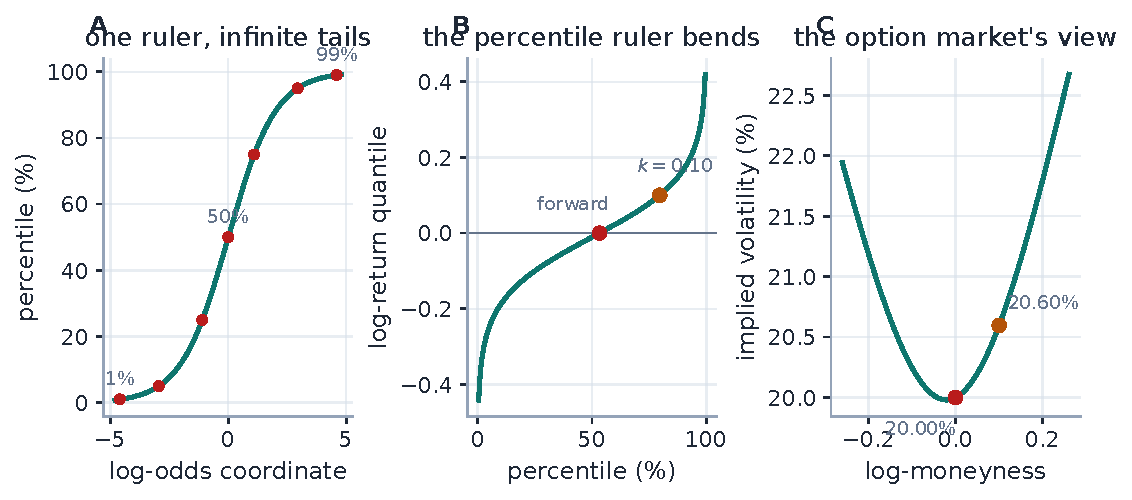
\includegraphics[width=0.98\textwidth]{fig_lqd_fresh_ruler.pdf}
\caption{\textbf{The percentile ruler in one exact toy.}
Left: the logistic score turns percentiles into an unbounded coordinate.
Middle: a constant-speed ruler maps that score to log return; the marked
forward and 10\% log-strike locate the two roots used in pricing.
Right: the same law is seen by the desk as an implied-volatility smile.  The
ATM volatility is exactly \lqdfreshtoyatm\%, while the $k=0.10$ point is
\lqdfreshtoyivten\%.  One random rank has become a complete option slice.}
\label{fig:ruler}
\end{figure}

%======================================================================
\section{The centering trade and the right-tail credit limit}
\label{sec:center}

The raw ruler $b$ has an arbitrary origin.  Option pricing does not: in forward
units the asset must have mean one.  Since $Y=e^{m+b(Z)}$, the unique centering
shift is
\begin{equation}
m=-\log\int_{-\infty}^{\infty}e^{b(z)}\rho(z)\,\dd z.
\label{eq:martingale_shift}
\end{equation}
Whenever this integral is finite,
\begin{equation}
\E[e^X]
=e^m\int_{-\infty}^{\infty}e^{b(z)}\rho(z)\,\dd z=1.
\label{eq:martingale_check}
\end{equation}
The shift changes location, not shape: $x'(z)=v(z)$ before and after
normalization.

\subsection{One hard inequality}

The two endpoint speeds are
\begin{equation}
\lambda_-=e^{h(0)},\qquad \lambda_+=e^{h(1)}.
\label{eq:endpoint_speeds}
\end{equation}
Because $h$ is a polynomial and
$\Lambda(z)=O(e^z)$ on the left while $1-\Lambda(z)=O(e^{-z})$ on the right,
\begin{align}
b(z)&=\lambda_-z+\delta_-+O(e^z),
&&z\to-\infty, \label{eq:left_b_asymptotic}\\
b(z)&=\lambda_+z+\delta_++O(e^{-z}),
&&z\to+\infty, \label{eq:right_b_asymptotic}
\end{align}
for finite constants $\delta_\pm$.  Combining these expressions with
\eqref{eq:logistic_tails}, the integrand in \eqref{eq:martingale_shift} behaves
as
\begin{equation}
e^{b(z)}\rho(z)\sim
\begin{cases}
C_-e^{(1+\lambda_-)z},&z\to-\infty,\\
C_+e^{-(1-\lambda_+)z},&z\to+\infty.
\end{cases}
\label{eq:normalizer_tails}
\end{equation}
The left tail always integrates because $\lambda_->0$.  The right tail
integrates exactly when $\lambda_+<1$.

\begin{proposition}[Finite-forward criterion]
\label{prop:finite_forward}
The construction in \eqref{eq:central_model} admits a finite martingale shift
if and only if
\begin{equation}
\lambda_+<1.
\label{eq:hard_wall}
\end{equation}
At $\lambda_+=1$ the normalizer diverges; this is a hard boundary, not a
calibration preference.
\end{proposition}

\begin{proof}
Equation \eqref{eq:normalizer_tails} makes the left integral finite for every
positive $\lambda_-$.  The right integral is comparable to
$\int^\infty e^{-(1-\lambda_+)z}\dd z$, which is finite precisely for
$\lambda_+<1$.  Equation \eqref{eq:martingale_shift} then gives the unique
finite translation.
\end{proof}

\begin{caution}
Approaching the wall is legal but expensive.  As $\lambda_+\uparrow1$, far
right states carry more and more of the mean.  The normalizer, tail quadrature,
price evaluation, and parameter sensitivities become numerically ill
conditioned before the mathematical boundary is reached.  Production
therefore adds a soft turn ahead of the hard wall and rejects
$\lambda_+\ge1-10^{-6}$ as a numerical safety buffer.  Neither control changes
the mathematical boundary at one.
\end{caution}

\subsection{The density falls out of the ruler}

Since $x'(z)=v(z)>0$ and $x(z)\to\pm\infty$, the map $x$ is an increasing
bijection.  Therefore
\begin{equation}
F_X(x(z))=\Lambda(z),\qquad
f_X(x(z))=\frac{\rho(z)}{v(z)}>0.
\label{eq:density_x}
\end{equation}
For the normalized asset,
\begin{equation}
f_Y(e^{x(z)})
=\frac{\rho(z)}{e^{x(z)}v(z)}>0.
\label{eq:density_y}
\end{equation}
Let $\widetilde c(y)=\E[(Y-y)^+]$ for a strike $y>0$.  Differentiation in
strike gives
\begin{equation}
\widetilde c'(y)=-\Prob(Y>y),\qquad
\widetilde c''(y)=f_Y(y)\ge0.
\label{eq:butterfly_derivatives}
\end{equation}
So the slice is decreasing and convex in \emph{strike}.  Convexity is not
asserted in log-strike $k$, where a change of variable contributes extra
terms.

\begin{proposition}[One-expiry static arbitrage]
\label{prop:butterfly}
If $h$ is finite and $\lambda_+<1$, the normalized call curve has the correct
boundaries, obeys put--call parity, and is strictly convex at every positive
strike.  In particular, every continuous butterfly spread has non-negative
value.
\end{proposition}

\begin{proof}
The construction gives $Y>0$ and $\E[Y]=1$.  Thus
$\widetilde c(0)=1$, $\widetilde c(y)\to0$ as $y\to\infty$, and
$(1-y)^+\le\widetilde c(y)\le1$.  Equation
\eqref{eq:butterfly_derivatives} supplies monotonicity and convexity.  Applying
the same law to puts yields $\widetilde c(y)-\widetilde p(y)=1-y$.
\end{proof}

\begin{figure}[H]
\centering
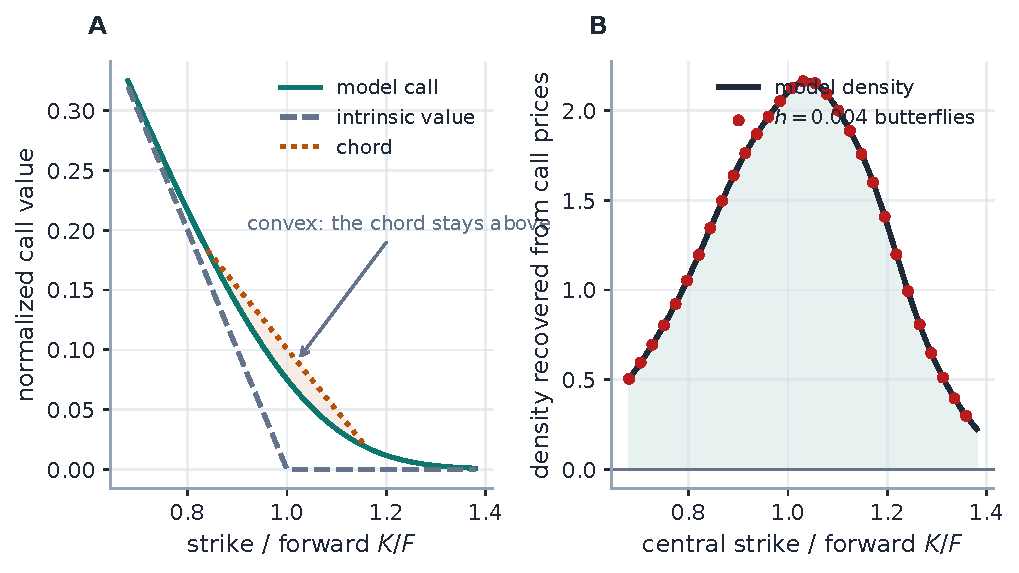
\includegraphics[width=0.96\textwidth]{fig_lqd_fresh_butterfly.pdf}
\caption{\textbf{Butterfly freedom is visible in price space.}
The left panel places the call above intrinsic value and below every secant
chord required by convexity.  The right panel recovers the continuous asset
density and compares it with discrete butterfly estimates.  In this audit the
minimum recovered density over the sampled window is
\lqdfreshminbutterfly, and the maximum relative discretization discrepancy on
that grid is \lqdfreshbutterflyrelerr\%.}
\label{fig:butterfly}
\end{figure}

%======================================================================
\section{A call is two tail ledgers}
\label{sec:ledger}

The probability law is now complete, but a trader wants a price.  Define the
upper asset-share ledger
\begin{equation}
G(z)=\int_z^\infty e^{x(t)}\rho(t)\,\dd t.
\label{eq:upper_share}
\end{equation}
It records how much of the mean-one asset is carried by states whose logistic
score exceeds $z$.  It starts at one, ends at zero, and satisfies
\begin{equation}
G'(z)=-e^{x(z)}\rho(z).
\label{eq:upper_share_derivative}
\end{equation}

For a log-strike $k$, let $z_k$ be the unique root
\begin{equation}
x(z_k)=k,\qquad p_k=\Lambda(z_k).
\label{eq:strike_root}
\end{equation}
Splitting the payoff gives
\begin{align}
c(k)
&=\int_{z_k}^{\infty}
  \bigl(e^{x(z)}-e^k\bigr)\rho(z)\,\dd z \notag\\
&=G(z_k)-e^k\bigl(1-p_k\bigr).
\label{eq:call_ledger}
\end{align}
This formula has a desk interpretation:
\begin{itemize}[leftmargin=1.4em]
\item $G(z_k)$ is the asset delivered in exercised states;
\item $e^k(1-p_k)$ is the strike bill paid in those states.
\end{itemize}
The call is the asset tail minus the cash tail.  No volatility interpolation is
involved.

\subsection{A complete trade ticket}

\begin{example}[title={A six-month call at $k=0.10$}]
\label{ex:call_ticket}
Take the constant-speed model calibrated to exactly
\lqdfreshtoyatm\% ATM volatility at active variance time
$\tau=\lqdfreshtoyexpiry$.  Its speed is
$s=\lqdfreshtoyscale$ and its martingale shift is
$m=\lqdfreshtoymu$.  At $k=0.10$, the exercise percentile is
$p_k=\lqdfreshtoyuten$ and the normalized strike is
$e^k=\lqdfreshtoystriketen$.  The asset ledger is
$G(z_k)=\lqdfreshtoyshareten$; the cash ledger is
$e^k(1-p_k)=\lqdfreshtoycashten$.  Their difference is
\[
c(0.10)
=\lqdfreshtoyshareten-\lqdfreshtoycashten
=\lqdfreshtoycallten
       =\lqdfreshtoycalltenpct\%\ \text{of forward}.
\]
Black inversion reports \lqdfreshtoyivten\%.  The price is primary; the
volatility is its market label.
\end{example}

The put ledger is obtained from the lower tail, but it need not be computed
separately.  Writing its price as $c_{\mathrm{put}}(k)$, mean-one
normalization gives
\begin{equation}
c(k)-c_{\mathrm{put}}(k)=1-e^k.
\label{eq:parity}
\end{equation}
It also supplies a useful implementation test: price calls from the upper
tail, recover puts by parity, and verify that a direct lower-tail calculation
agrees.

\subsection{Digital and density from the same root}

The root motion cancels when differentiating the payoff integral, because the
payoff is zero at the exercise boundary.  Consequently
\begin{equation}
c'(k)=-e^k(1-p_k),
\label{eq:call_first_k}
\end{equation}
and one more derivative gives
\begin{equation}
c''(k)
=-e^k(1-p_k)+
e^k\frac{\rho(z_k)}{v(z_k)}.
\label{eq:call_second_k}
\end{equation}
The combination
\begin{equation}
e^{-k}\bigl(c''(k)-c'(k)\bigr)
=\frac{\rho(z_k)}{v(z_k)}
=f_X(k)
\label{eq:density_from_k}
\end{equation}
recovers the log-return density.  In strike coordinates this is the
Breeden--Litzenberger identity \cite{breedenlitzenberger}; in the transport
coordinate it is one division.

\begin{heuristic}
The function $G$ will recur twice.  In \cref{sec:jacobian}, its parameter
derivatives give the calibration Jacobian without differentiating $z_k$.  In
\cref{sec:calendar}, $G$ becomes the integrated-quantile curve that orders
expiries.  Pricing, differentiation, and calendars are three uses of the same
ledger.
\end{heuristic}


\section{The constant-speed audit}
\label{sec:constant}

Before trusting a flexible model, make it solve a case that fits on one page.
Set
\begin{equation}
h(p)=\log s,\qquad 0<s<1.
\label{eq:constant_speed}
\end{equation}
Then $v(z)=s$, $b(z)=sz$, and the logistic moment-generating function gives
\begin{equation}
\E[e^{sZ}]=\frac{\pi s}{\sin(\pi s)}.
\label{eq:logistic_mgf}
\end{equation}
The martingale shift and transport are therefore
\begin{equation}
m=-\log\frac{\pi s}{\sin(\pi s)},\qquad x(z)=m+sz.
\label{eq:constant_transport}
\end{equation}
The condition $s<1$ is simultaneously the domain of the moment in
\eqref{eq:logistic_mgf} and the hard right-tail condition
\eqref{eq:hard_wall}.

\begin{example}[title={An exact 20\% ATM unit check}]
\label{ex:constant_unit}
Solving the one-dimensional equation
\[
2\PhiN\!\left(\frac{0.20\sqrt{0.50}}{2}\right)-1
=c(0;s)
\]
gives $s=\lqdfreshtoyscale$.  Equation
\eqref{eq:constant_transport} then gives
$m=\lqdfreshtoymu$, and the forward lies at percentile
\lqdfreshtoyuatmpct\%, not at the median.  The latter is not a bug:
martingale centering occurs in \emph{price}, so the log return usually has a
negative location shift.
\begin{center}
\lqdfreshtoytable
\end{center}
\end{example}

%======================================================================


The constant-speed law is not a flat Black smile.  It is a log-logistic
distribution rescaled to mean one, so its wing moments are finite only over a
strip.  Its purpose is more valuable than realism: every integration,
root-finding, normalization, price, and implied-vol inversion path can be
checked against a transparent one-parameter model.

%======================================================================
\section{The ATM microscope}
\label{sec:atm}

At the money, three distributional facts replace a neighbourhood of finite
differences.  Let $z_*$ solve $x(z_*)=0$ and define
\begin{equation}
p_*=\Lambda(z_*),\qquad
f_*=\frac{\rho(z_*)}{v(z_*)}=f_X(0).
\label{eq:atm_percentile_density}
\end{equation}
Equations \eqref{eq:call_ledger}--\eqref{eq:call_second_k} give
\begin{equation}
c_0=G(z_*)-(1-p_*),\qquad
c'_0=-(1-p_*),\qquad
c''_0=f_*-(1-p_*).
\label{eq:atm_three_facts}
\end{equation}
The ATM price sets level, the exercise percentile sets the digital, and the
local compression of the ruler sets density.

\subsection{Pass those facts through Black}

Let $B(k,w)$ denote the normalized Black call with total variance $w$, and let
$w(k)$ solve
\begin{equation}
B(k,w(k))=c(k).
\label{eq:black_inversion}
\end{equation}
At $k=0$, put
\begin{equation}
a=\PhiN^{-1}\!\left(\frac{1+c_0}{2}\right),\qquad
w_0=4a^2,\qquad n=\phin(a),\qquad
\Delta=p_*-\PhiN(a).
\label{eq:atm_black_symbols}
\end{equation}
Implicit differentiation produces unusually compact identities:
\begin{align}
w'_0&=\frac{2\sqrt{w_0}}{n}\,\Delta,
\label{eq:atm_w1}\\
w''_0&=\frac{2\sqrt{w_0}}{n}\,f_*
       -2+
       \left(\frac{1}{2w_0}+\frac18\right)(w'_0)^2.
\label{eq:atm_w2}
\end{align}
The derivation is recorded in \cref{app:numerics}; the interpretation belongs
here.  Total-variance skew is exactly a \emph{digital mismatch}: $p_*$ is the
model percentile of the forward, while $\PhiN(a)$ is the corresponding
percentile under the flat-Black law with the same ATM option price.  Curvature
adds the local-density mismatch and a necessary nonlinear skew correction.

If $\tau$ is the active variance time and
$\sigma(k)=\sqrt{w(k)/\tau}$, then
\begin{align}
\sigma_0&=\sqrt{\frac{w_0}{\tau}},
\label{eq:atm_vol}\\
\sigma'_0&=\frac{\Delta}{n\sqrt{\tau}},
\label{eq:atm_skew}\\
\sigma''_0&=\frac{1}{\sqrt{\tau}}
\left[
\frac{f_*}{n}-\frac{1}{\sqrt{w_0}}
+\frac{\sqrt{w_0}}{4}\left(\frac{\Delta}{n}\right)^2
\right].
\label{eq:atm_curvature}
\end{align}
These are exact identities for the continuous slice.  They are
semi-analytic, not elementary coefficient formulas: $z_*$ and $c_0$ still
come from monotone inversion and quadrature.

\begin{proposition}[ATM information content]
\label{prop:atm}
Once the martingale law is built, ATM level, log-strike skew, and log-strike
curvature depend only on $(c_0,p_*,f_*)$ and the variance clock $\tau$.
No neighbouring implied-volatility quotes are required.
\end{proposition}

\begin{proof}
At ATM, $B(0,w)=2\PhiN(\sqrt w/2)-1$, which gives
\eqref{eq:atm_black_symbols}.  The Black partial
$B_w(0,w)=\phin(\sqrt w/2)/(2\sqrt w)$ together with
\eqref{eq:atm_three_facts} yields \eqref{eq:atm_w1}.  Differentiating
$B(k,w(k))=c(k)$ twice and simplifying the ATM Black partials gives
\eqref{eq:atm_w2}.  The chain rule for $\sigma=\sqrt{w/\tau}$ gives
\eqref{eq:atm_vol}--\eqref{eq:atm_curvature}.
\end{proof}

\begin{example}[title={The digital explains skew before any regression does}]
Suppose the model forward percentile $p_*$ lies below the matched-Black
percentile $\PhiN(a)$.  Then $\Delta<0$, so
\eqref{eq:atm_skew} says the implied-volatility skew is negative.  The
statement does not rely on a three-point slope, a fitted parabola, or a small
bump size.  It is an exact comparison of two digitals.
\end{example}

%======================================================================
\section{The part of the smile no quote sees}
\label{sec:tails}

Liquid quotes constrain the body.  Extrapolation is governed by what the ruler
does as ranks approach zero and one.  From
\eqref{eq:left_b_asymptotic}--\eqref{eq:right_b_asymptotic},
\begin{equation}
\Prob(X>x)\sim K_+e^{-x/\lambda_+},\qquad
\Prob(X<x)\sim K_-e^{x/\lambda_-},
\label{eq:x_tail_probs}
\end{equation}
for positive constants $K_\pm$.  Equivalently, $Y=e^X$ has power tails:
\begin{equation}
\Prob(Y>y)\sim K_+y^{-1/\lambda_+},\qquad
\Prob(Y<y)\sim K_-y^{1/\lambda_-}.
\label{eq:y_tail_probs}
\end{equation}

\subsection{Moment budget}

The same endpoint comparison gives the complete moment strip
\begin{equation}
\E[e^{rX}]<\infty
\quad\Longleftrightarrow\quad
-\frac{1}{\lambda_-}<r<\frac{1}{\lambda_+}.
\label{eq:moment_strip}
\end{equation}
For the asset $Y$, the critical Lee moments are
\begin{equation}
\pi_+=\frac{1}{\lambda_+}-1,\qquad
\pi_-=\frac{1}{\lambda_-}.
\label{eq:critical_moments}
\end{equation}
The first says how many moments beyond the forward survive on the right; the
second says how many inverse moments survive on the left.

Lee's moment formula \cite{lee} uses the map
\begin{equation}
\Psi(q)=2-4\left(\sqrt{q^2+q}-q\right).
\label{eq:lee_map}
\end{equation}
For total implied variance, the wing limsups are
\begin{equation}
\limsup_{k\to\infty}\frac{w(k)}{k}=\Psi(\pi_+),\qquad
\limsup_{k\to-\infty}\frac{w(k)}{|k|}=\Psi(\pi_-).
\label{eq:lee_limsup}
\end{equation}
Substituting \eqref{eq:critical_moments} yields direct speed-to-slope formulas:
\begin{align}
\beta_+
&=\frac{2\lambda_+}
        {\bigl(1+\sqrt{1-\lambda_+}\bigr)^2},
&&0<\lambda_+<1, \label{eq:beta_right}\\
\beta_-
&=\frac{2\lambda_-}
        {\bigl(1+\sqrt{1+\lambda_-}\bigr)^2},
&&\lambda_->0. \label{eq:beta_left}
\end{align}
For small endpoint speeds, $\beta_\pm\sim\lambda_\pm/2$.  As the right speed
approaches the hard wall, $\beta_+\to2$.

\begin{caution}
Lee's theorem itself gives the limsup statement
\eqref{eq:lee_limsup}.  The polynomial endpoint expansion here produces
regular power tails, so regular-variation tail--wing refinements
\cite{benaimfriz} upgrade the wing rates to ordinary limits.  When only Lee's
moment result is being invoked, the careful word is \emph{limsup}.
\end{caution}

\begin{figure}[H]
\centering
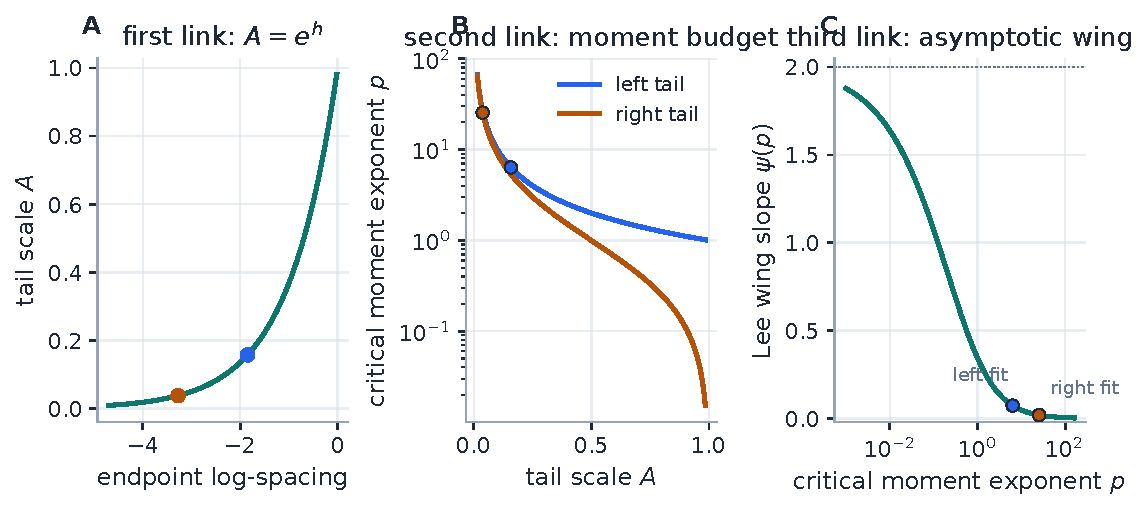
\includegraphics[width=0.98\textwidth]{fig_lqd_fresh_tails.pdf}
\caption{\textbf{The endpoint is an extrapolation forecast.}
Left: the speed profile settles to two endpoint values.  Centre: those values
are inverse moment budgets through \eqref{eq:critical_moments}.  Right: the
moment budgets map to Lee total-variance slopes.  The marked production fit has
$(\lambda_-,\lambda_+)=(\lqdfreshspxAL,\lqdfreshspxAR)$ and
$(\beta_-,\beta_+)=(\lqdfreshspxbetaL,\lqdfreshspxbetaR)$.}
\label{fig:tails}
\end{figure}

\begin{example}[title={The right endpoint has a balance-sheet meaning}]
\label{ex:tail_stress}
For the SPX-like fit in \cref{sec:screen}, the right speed is
$\lambda_+=\lqdfreshspxAR$.  Hence the model retains moments
$\E[Y^{1+q}]$ for $q<1/\lqdfreshspxAR-1$ and predicts a right-wing Lee slope
of \lqdfreshspxbetaR.  Moving a high-order coefficient can leave quoted
strikes nearly unchanged yet alter $h(1)$, the critical moment boundary, and
the far wing.  A small in-window residual is therefore not an extrapolation
diagnostic.
\end{example}

%======================================================================
\section{Put the quote screen back in}
\label{sec:screen}

Only now do we return to market quotes.  The model provides arbitrage-safe
prices; Black inversion merely expresses those prices in familiar units.
For total variance $w$, the normalized Black call is
\begin{equation}
B(k,w)=\PhiN(d_+)-e^k\PhiN(d_-),\qquad
d_\pm=-\frac{k}{\sqrt w}\pm\frac{\sqrt w}{2}.
\label{eq:black_call}
\end{equation}
At quote $i$, target price $B(k_i,w_i^{\mathrm{mkt}})$ is compared with model
price $c(k_i;\theta)$.  A useful core residual is
\begin{equation}
r_i(\theta)=
\omega_i^{1/2}
\frac{c(k_i;\theta)-B(k_i,w_i^{\mathrm{mkt}})}
     {\mathrm{Vega}_i+\eta}.
\label{eq:vega_residual}
\end{equation}
Here $\eta>0$ prevents tiny far-wing vegas from acquiring absurd weight.
With normalized Black vega
$\mathrm{Vega}_i=\phin(d_{+,i})\sqrt{\tau}$, $r_i$ is approximately an
implied-volatility error.

\subsection{What the objective is allowed to prefer}

The residual stack adds controls, each with a distinct economic meaning:
\begin{itemize}[leftmargin=1.4em]
\item bid--ask bands can replace point targets with zero hinge cost inside the
  spread, while retaining a gentle midpoint anchor;
\item a ridge on modes $n\ge4$ discourages oscillatory speed profiles that
  sparse quotes cannot identify;
\item a one-sided soft barrier turns the optimizer away before
  $\lambda_+=1$;
\item optional priors stabilize weakly identified tails or preserve continuity
  with the previous fit;
\item optional calendar rows penalize crossings of upper-share ledgers;
\item optional log-contract and ATM/RR/BF operator rows express desk views.
\end{itemize}
The hard martingale wall remains hard.  Every other row is a weighted modelling
choice and should be reported as such.

\begin{perfbox}
Production prices in the native coordinate.  It tabulates $x(z)$ and $G(z)$
once, solves all strike roots monotonically, and evaluates each call from
\eqref{eq:call_ledger}.  This is faster and numerically calmer than integrating
each payoff from scratch.
\end{perfbox}

\subsection{A deterministic SPX-like approximation case}

The first stress case uses a smooth skewed target sampled at
\lqdfreshspxnquotes\ strikes and fits an order-\lqdfreshspxorder\ LQD slice with
the production calibrator.  It is a capacity and implementation test, not a
claim about a live market or a trading signal.

\begin{figure}[H]
\centering
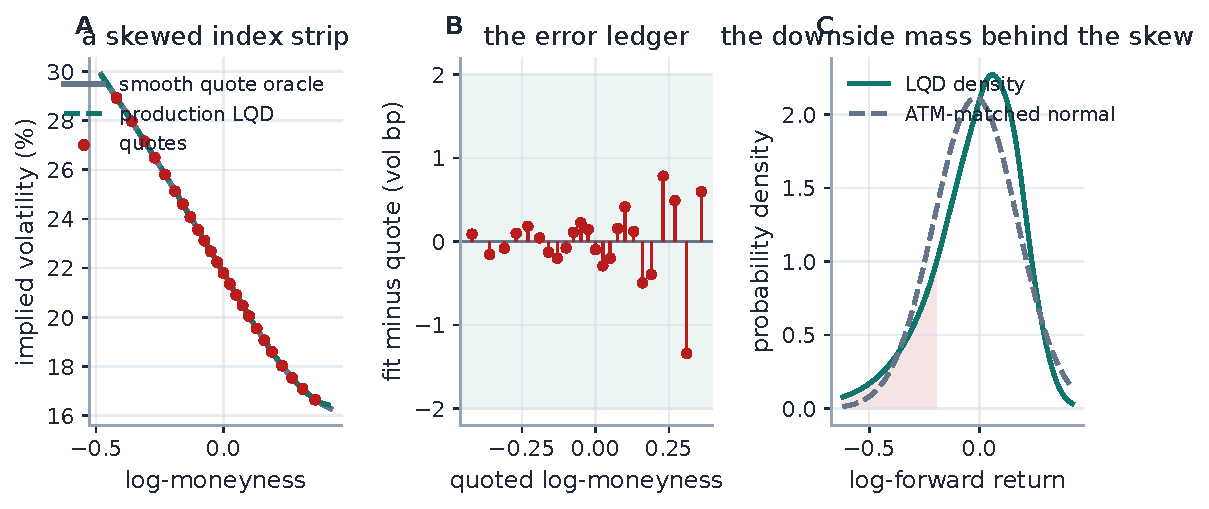
\includegraphics[width=0.98\textwidth]{fig_lqd_fresh_spx.pdf}
\caption{\textbf{A quote screen, its residual ledger, and the law underneath.}
Left: the order-\lqdfreshspxorder\ production fit overlays the deterministic
SPX-like target.  Centre: all residuals remain inside a narrow
volatility-basis-point band; maximum and RMS errors are
\lqdfreshspxmaxerr\ and \lqdfreshspxrmserr\ bp.  Right: the fitted return
density is compared with an ATM-matched normal, making the downside allocation
of probability visible.}
\label{fig:spx}
\end{figure}

\begin{example}[title={Read the fit in three coordinate systems}]
\label{ex:spx}
The optimizer terminates in \lqdfreshspxnfev\ function evaluations.  The quote
screen reports ATM volatility \lqdfreshspxatm\%, skew
\lqdfreshspxskew, and curvature \lqdfreshspxcurvature.  The distribution
reports endpoint speeds
$(\lqdfreshspxAL,\lqdfreshspxAR)$ and martingale error
\lqdfreshspxmart.  The terminal log contract reports a
log-contract-implied volatility of \lqdfreshspxvarswap\%.  None of these views
replaces the others: quotes measure fit, endpoint speeds measure extrapolation,
and the density shows where probability actually landed.
\end{example}

\section{How to move level without wrecking shape}
\label{sec:handles}

Raw polynomial coefficients are efficient calibration coordinates and poor
conversation.  A trader asks for more level with skew unchanged, not for a
bump to the fourth Legendre coefficient.  Let
\begin{equation}
H(\theta)=
\begin{pmatrix}
w_0(\theta)\\
\sigma'_0(\theta)\\
\sigma''_0(\theta)
\end{pmatrix},
\qquad
D=\frac{\partial H}{\partial\theta}.
\label{eq:handle_map}
\end{equation}
The internal production chart uses $w_0$ in its first coordinate.  The
screen-facing level is $\sigma_0$, and at fixed $\tau$ the two charts are
locally equivalent through $w_0=\tau\sigma_0^2$.  At a regular point, $D$ has
row rank three.  The minimum-norm first-order move that changes handles by
$\delta H$ is
\begin{equation}
\delta\theta_{\mathrm{primary}}
=D\T(DD\T)^{-1}\delta H.
\label{eq:primary_move}
\end{equation}
Any vector in $\ker D$ is a first-order shape move: it changes the smile while
leaving ATM level, skew, and curvature fixed to first order.

\begin{assumption}[Regular handle point]
\label{ass:regular}
The parameter vector lies strictly inside $\lambda_+<1$, the ATM option has
non-negligible vega, and $D$ has row rank three.  Near a rank loss, the
pseudoinverse is a warning signal rather than a trading control.
\end{assumption}

The linear move is local.  A finite requested shift can be attempted with
Newton retargeting on the exact handles
\eqref{eq:atm_vol}--\eqref{eq:atm_curvature}.  The current routine is not a
globally feasible map: an intermediate iterate can meet the martingale wall,
and the solve can fail near a singular chart.  This distinction matters: a
linear chart is a compass, not a teleport.

\begin{figure}[H]
\centering
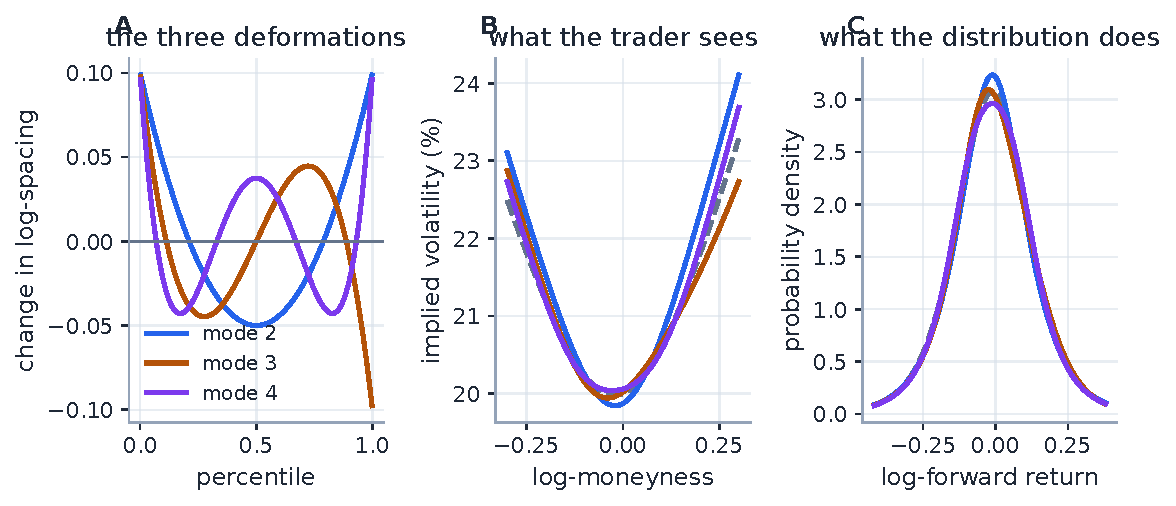
\includegraphics[width=0.98\textwidth]{fig_lqd_fresh_modes.pdf}
\caption{\textbf{What low polynomial modes actually move.}
Each panel is one view --- log-speed, implied volatility, or return density ---
and overlays the same three controlled perturbations.  Broad modes move level
or tilt; higher curvature redistributes probability more locally.  The panels
explain why coefficient orthogonality is useful but does not make coefficients
into trader handles.}
\label{fig:modes}
\end{figure}

\begin{example}[title={Primary move versus shape move}]
With order $N=9$, there are ten polynomial coefficients but only three ATM
handles.  Under \cref{ass:regular}, the primary subspace has dimension three
and the local shape nullspace has dimension seven.  A calibration can therefore
match the same ATM level, skew, and curvature with materially different wing
or density shapes.  Quotes and regularization decide which member of that
seven-dimensional family is acceptable.
\end{example}

%======================================================================
\section{The root that disappears}
\label{sec:jacobian}

Calibration speed depends on derivatives.  A naive implementation bumps every
coefficient, rebuilds the martingale shift, resolves every strike root, and
reprices every option.  The transport reveals a cleaner route.

Write the profile in any affine coefficient chart,
\begin{equation}
h_\theta(p)=\sum_j\theta_j\phi_j(p).
\label{eq:affine_chart}
\end{equation}
The raw-ruler sensitivity is
\begin{equation}
r_j(z)=\frac{\partial b(z)}{\partial\theta_j}
=\int_0^z v(t)\phi_j(\Lambda(t))\,\dd t.
\label{eq:raw_sensitivity}
\end{equation}
Differentiate the mean-one identity.  Since
$1=\int e^{x(z)}\rho(z)\dd z$,
\begin{equation}
\frac{\partial m}{\partial\theta_j}
=-\int_{-\infty}^{\infty}e^{x(t)}r_j(t)\rho(t)\,\dd t,
\label{eq:shift_sensitivity}
\end{equation}
and hence
\begin{equation}
x_j(z):=\frac{\partial x(z)}{\partial\theta_j}
=r_j(z)-
\int_{-\infty}^{\infty}e^{x(t)}r_j(t)\rho(t)\,\dd t.
\label{eq:x_sensitivity}
\end{equation}
Define the corresponding upper-share sensitivity
\begin{equation}
G_j(z)=\int_z^\infty e^{x(t)}x_j(t)\rho(t)\,\dd t.
\label{eq:G_sensitivity}
\end{equation}

\begin{theorem}[Envelope cancellation]
\label{thm:envelope}
At fixed log-strike $k$ and an interior admissible parameter vector,
\begin{equation}
\frac{\partial c(k;\theta)}{\partial\theta_j}=G_j(z_k).
\label{eq:analytic_price_jacobian}
\end{equation}
The derivative of the implicit strike root $z_k$ is not needed.
\end{theorem}

\begin{proof}
Differentiate \eqref{eq:call_ledger}.  Terms involving the moving root combine
to
\[
\left[G'(z_k)+e^k\rho(z_k)\right]
\frac{\partial z_k}{\partial\theta_j}.
\]
But \eqref{eq:upper_share_derivative} and $x(z_k)=k$ imply
$G'(z_k)=-e^k\rho(z_k)$.  The bracket vanishes.  The remaining fixed-boundary
term is exactly \eqref{eq:G_sensitivity}.
\end{proof}

This is an envelope theorem in trading clothes.  Moving the exercise boundary
has no first-order value because the option payoff is zero at that boundary.
The expensive implicit derivative disappears for an economic reason, not an
algebraic accident.

\begin{figure}[H]
\centering
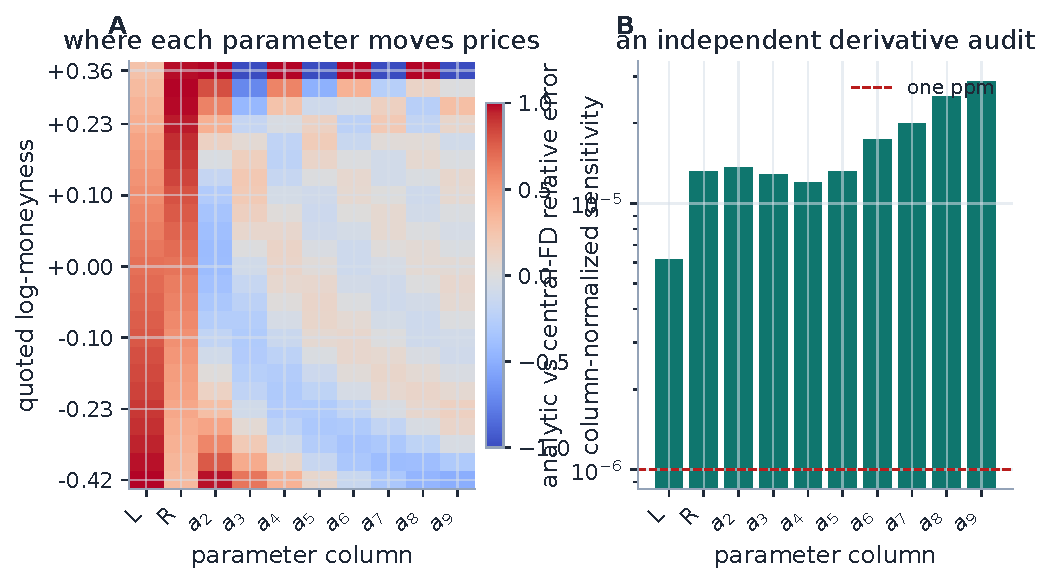
\includegraphics[width=0.98\textwidth]{fig_lqd_fresh_jacobian.pdf}
\caption{\textbf{The analytic price Jacobian under audit.}
Left: the production sensitivities for \lqdfreshjacnparams\ parameters are
compared with central finite differences across strikes.  Right: normalized
column errors remain below \lqdfreshjacmaxrel.  The residual discrepancy is
the expected finite-grid/interpolation error, not a missing strike-root term.}
\label{fig:jacobian}
\end{figure}

\begin{caution}
The continuous identity is exact under dominated differentiation in an
interior neighbourhood.  Production tabulates and interpolates $x$ and $G$
separately, so off-grid algebra is not bitwise exact.  Sensitivities also grow
poorly conditioned near $\lambda_+=1$.  Finite-difference audits remain a
necessary test even when finite differences are no longer the main algorithm.
\end{caution}

%======================================================================
\section{When probability chooses two landing zones}
\label{sec:event}

Positive density does not mean unimodal density.  If the ruler moves slowly in
two separated regions, probability ranks bunch into two return zones.  This is
useful around discrete events and dangerous when caused by overfitting.

To make that distinction visible, the second deterministic case starts from
an asymmetric two-component event law.  Its left component carries
\lqdfresheventweightleft\% weight and is centred at
\lqdfresheventmeanleft; the right component is centred at
\lqdfresheventmeanright.  We sample \lqdfresheventnquotes\ option quotes and
fit the highest supported production order, $N=\lqdfresheventorder$.

\begin{figure}[H]
\centering
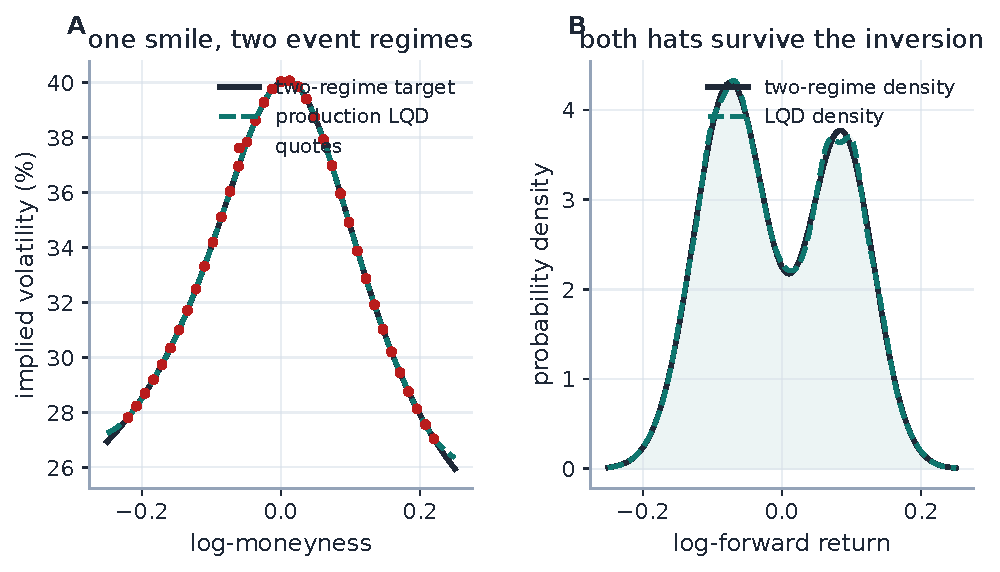
\includegraphics[width=0.98\textwidth]{fig_lqd_fresh_event.pdf}
\caption{\textbf{An adversarial event case.}
Left: the order-\lqdfresheventorder\ production slice approximates the
event-shaped implied-volatility target with maximum and RMS quote errors
\lqdfresheventmaxerr\ and \lqdfresheventrmserr\ volatility bp.  Right: the
recovered density visibly selects two landing zones.  The fit tests whether a
positive transport family can express bimodality; it does not certify that the
second mode is economically real.}
\label{fig:event}
\end{figure}

\begin{example}[title={Positive is guaranteed; plausible is judged}]
\label{ex:event}
The fit has endpoint speeds
$(\lqdfresheventAL,\lqdfresheventAR)$ and martingale error
\lqdfresheventmart.  Its density cannot be negative, regardless of order.
Yet a second mode may reflect a genuine scheduled jump, sparse quotes, a loose
high-order ridge, or stale prices.  Static arbitrage supplies a floor for model
quality, not a complete economic opinion.
\end{example}

The example also explains why order is a risk control.  Raising $N$ expands
approximation capacity and creates more ways to hide oscillation between
quotes.  High order is justified when the data or prior information can
identify the extra structure.  Otherwise it is merely freedom with a polished
residual.

%======================================================================
\section{Stacking expiry engines}
\label{sec:calendar}

Each expiry engine is butterfly-free on its own.  A surface must also avoid a
shorter-dated call being more expensive than a longer-dated call at the same
normalized strike.  The right object is not the log-return mean or variance;
it is convex order for the normalized asset.

Under deterministic proportional carry and a consistent mean-one forward
normalization, write for expiry $T$ the percentile map
\begin{equation}
y_T(p)=
\exp\!\left(
x_T\!\left(\log\frac{p}{1-p}\right)
\right),\qquad 0<p<1,
\label{eq:asset_quantile}
\end{equation}
and its upper integrated percentile curve
\begin{equation}
\mathcal G_T(p)=\int_p^1y_T(r)\,\dd r.
\label{eq:integrated_quantile}
\end{equation}
The substitution $r=\Lambda(z)$ reveals the promised identity
\begin{equation}
\mathcal G_T(p)=G_T\!\left(\log\frac{p}{1-p}\right).
\label{eq:G_identity}
\end{equation}
The price ledger is already the calendar ledger.

\subsection{Why ordering the ledgers orders every call}

At normalized strike $y$,
\begin{equation}
\widetilde c_T(y)
=\sup_{0\le p\le1}
\left\{\mathcal G_T(p)-(1-p)y\right\}.
\label{eq:call_conjugate}
\end{equation}
A maximizing percentile is associated with the exercise threshold
$y_T(p)=y$.  Conversely,
\begin{equation}
\mathcal G_T(p)
=\inf_{y\ge0}
\left\{\widetilde c_T(y)+(1-p)y\right\}.
\label{eq:G_conjugate}
\end{equation}
These conjugate relations prove the ordering result directly; they are the
integrated-quantile form of standard convex order
\cite{hardylittlewoodpolya,shakedshanthikumar}.

\begin{theorem}[Calendar order in the native ledger]
\label{thm:calendar}
Let $Y_1$ and $Y_2$ be positive integrable variables with mean one, and for a
general law let $y_i(p)$ denote its left-continuous generalized quantile.
Then
\begin{equation}
Y_1\le_{\mathrm{cx}}Y_2
\quad\Longleftrightarrow\quad
\mathcal G_1(p)\le\mathcal G_2(p)
\quad\text{for every }p\in[0,1].
\label{eq:convex_order}
\end{equation}
Equivalently, every normalized call on $Y_1$ is no more expensive than the
same-strike call on $Y_2$.
\end{theorem}

\begin{proof}
If the integrated percentiles are ordered, taking suprema in
\eqref{eq:call_conjugate} orders every call.  If every call is ordered, taking
infima in \eqref{eq:G_conjugate} orders every integrated percentile.  Equal
means supply equality at $p=0$, and both curves vanish at $p=1$.
\end{proof}

\begin{example}[title={A calendar crossing can hide between strikes}]
\label{ex:calendar}
Suppose two adjacent expiries satisfy
$\mathcal G_1(p_j)\le\mathcal G_2(p_j)$ at the quoted exercise percentiles but
cross between $p_j$ and $p_{j+1}$.  Quote-by-quote checks pass, yet
\cref{thm:calendar} implies that some unquoted strike has a negative calendar
spread.  A dense logit grid makes such a crossing harder to miss; only a
continuum certificate rules it out mathematically.
\end{example}

Production evaluates \eqref{eq:G_identity} on a finite logit grid and adds
finite-weight hinge residuals for negative gaps.  This is effective calendar
\emph{control}, not a structural guarantee.  It protects listed expiries at
sampled ranks; it does not certify every rank, arbitrary interpolation between
expiries, or models with inconsistent forward measures.

\subsection{The native log contract}

Because $P=\Lambda(Z)$ is uniform,
\begin{equation}
\E[X]=\int_0^1x\!\left(\log\frac{p}{1-p}\right)\dd p.
\label{eq:mean_log_return}
\end{equation}
For a mean-one positive asset, define the terminal log-contract quantity
\begin{equation}
w_{\log}=-2\E[X].
\label{eq:log_contract}
\end{equation}
This route integrates the constructed law directly.  It avoids extrapolating a
finite strike grid before evaluating the familiar option-strip replication
\cite{gatheral}.  The annualized display uses the active variance clock,
$\sigma_{\log}=\sqrt{w_{\log}/\tau}$.  The identity is exact for the terminal
log contract.  It equals the fair pathwise realized-variance strike under the
usual continuous-path replication assumptions; jumps introduce a correction,
and a terminal marginal alone cannot price realized variance.

%======================================================================
\section{The honest contract}
\label{sec:contract}

A good model note should end its sales pitch before the reader has to.  The
table below separates what follows from the mathematics from what is merely
encouraged by a calibration objective.

\begin{table}[H]
\centering
\caption{What the model promises, controls, and does not claim.}
\label{tab:contract}
\begin{tabular}{@{}p{0.27\textwidth}p{0.20\textwidth}p{0.45\textwidth}@{}}
\toprule
Property & Status & Precise statement\\
\midrule
Positive continuous density
& Structural
& $v>0$ makes $x$ increasing and \eqref{eq:density_x} positive.\\
Mean-one normalized asset
& Structural, conditional
& Exact after \eqref{eq:martingale_shift}, provided $\lambda_+<1$.\\
One-expiry butterfly freedom
& Structural
& Calls are convex in normalized strike, not necessarily in log-strike.\\
Tail moments and Lee rates
& Structural
& Endpoint speeds determine \eqref{eq:moment_strip} and
  \eqref{eq:beta_right}--\eqref{eq:beta_left}.\\
ATM level, skew, curvature
& Exact slice identities
& Equations \eqref{eq:atm_vol}--\eqref{eq:atm_curvature}; numerical
  quadrature and root solves are still required.\\
Calendar freedom
& Soft in production
& Exact if \eqref{eq:convex_order} holds for all ranks; production samples
  finitely and uses finite weights.\\
Unimodality or economic plausibility
& Not guaranteed
& Positive density can be oscillatory or multimodal.\\
Atoms and default mass
& Not represented directly
& A finite smooth speed produces a continuous positive law on $(0,\infty)$.\\
Parameter identification
& Not guaranteed
& Sparse quotes may leave tail and high-order directions weakly identified.\\
Dynamic arbitrage under stochastic carry
& Outside the slice theorem
& Marginal normalized convex order is not a full dynamic market model.\\
\bottomrule
\end{tabular}
\end{table}

\begin{invariant}
The durable mental model is short.  Draw a logistic rank.  Move it through a
positive-speed ruler.  Translate the ruler so the asset mean is one.  Price a
call as an upper asset share minus an upper cash bill.  Read extrapolation from
the two endpoint speeds.  Everything else is implementation, calibration, or
governance.
\end{invariant}


\appendix

%======================================================================
\section{Numerical construction and exact ATM algebra}
\label{app:numerics}

\subsection{A stable finite grid}

Production works on a finite logistic interval $[-z_{\max},z_{\max}]$.  On a
sorted grid $z_j$, it evaluates
\[
p_j=\Lambda(z_j),\qquad v_j=e^{h(p_j)},
\]
and integrates $v$ outward from the anchor $z=0$ to obtain $b_j$.  The
martingale integrand and upper-share integrand begin with the same array,
\[
a_j=e^{b_j}\rho(z_j).
\]
The normalizer is $M=\int a(z)\dd z$, the shift is $m=-\log M$, and the
normalized upper share is
\begin{equation}
G(z)=\frac{\int_z^\infty a(t)\dd t}{M}.
\label{eq:numerical_share}
\end{equation}
Computing numerator and denominator from the unshifted integrand is useful:
their potentially large common scale cancels.

The omitted tails are not set to zero.  From
\eqref{eq:left_b_asymptotic}--\eqref{eq:right_b_asymptotic}, their leading
integrals are exponential and can be added analytically.  For example, at a
right boundary $z_R$,
\begin{equation}
\int_{z_R}^\infty e^{b(z)}\rho(z)\,\dd z
\approx
\frac{e^{b(z_R)-z_R}}{1-\lambda_+},
\label{eq:right_tail_correction}
\end{equation}
while at a left boundary $z_L<0$,
\begin{equation}
\int_{-\infty}^{z_L} e^{b(z)}\rho(z)\,\dd z
\approx
\frac{e^{b(z_L)+z_L}}{1+\lambda_-}.
\label{eq:left_tail_correction}
\end{equation}
These are the leading production corrections.  They become ill conditioned
near the hard wall, as they should.

\subsection{Hermite interpolation and root solves}

The tabulated $x_j=m+b_j$ is strictly increasing.  Production uses piecewise
cubic Hermite interpolants supplied with the analytic nodal slopes
$x'=v$ and $G'=-e^x\rho$.  This gives fourth-order local accuracy, but it is
not a Fritsch--Carlson monotonicity guarantee \cite{fritschcarlson};
monotonicity between nodes is therefore a numerical audit on the chosen grid.
Strike inversion starts from a monotone linear-table seed and applies a small
fixed number of clipped Newton updates.

The finite-grid price is then \eqref{eq:call_ledger}.  Three routine audits
catch most errors:
\begin{enumerate}[leftmargin=1.6em]
\item verify $G(-z_{\max})$ plus its left correction is one to tolerance;
\item compare direct lower-tail puts with calls recovered from parity;
\item refine the grid and confirm that prices, densities, and Jacobians
converge together.
\end{enumerate}

\subsection{ATM Black derivatives}

For completeness, let $s=\sqrt w$ and
$d_\pm=-k/s\pm s/2$.  At fixed $w$,
\begin{equation}
B_k=-e^k\PhiN(d_-),\qquad
B_w=\frac{\phin(d_+)}{2s}.
\label{eq:black_first_partials}
\end{equation}
At $k=0$, with $a=s/2$ and $n=\phin(a)$,
\begin{align}
B_k&=\PhiN(a)-1, &
B_w&=\frac{n}{2s}, \label{eq:black_atm_first}\\
B_{kk}&=\frac{n}{s}+\PhiN(a)-1, &
B_{kw}&=\frac{n}{4s}, \label{eq:black_atm_second_a}\\
B_{ww}&=
-n\left(\frac{1}{16s}+\frac{1}{4s^3}\right).
\label{eq:black_atm_second_b}
\end{align}
Implicit differentiation gives
\begin{align}
w'_0&=\frac{c'_0-B_k}{B_w},\label{eq:implicit_w1}\\
w''_0&=
\frac{c''_0-B_{kk}-2B_{kw}w'_0-B_{ww}(w'_0)^2}{B_w}.
\label{eq:implicit_w2}
\end{align}
Substituting \eqref{eq:atm_three_facts} and
\eqref{eq:black_atm_first}--\eqref{eq:black_atm_second_b} simplifies to
\eqref{eq:atm_w1}--\eqref{eq:atm_w2}.  The terms linear in $w'_0$ cancel.

\subsection{Two clocks}

$T$ labels the expiry and governs discounting and forwards.  The quantity
$\tau$ annualizes total variance.  In the base configuration they coincide as
year fractions.  With an event clock, $\tau$ includes the scheduled-event
dilation used elsewhere in Vol-Fitter.  All Black vegas and annualized handles
must use the same active $\tau$ that produced the target total variances.

%======================================================================
\section{Production dictionary, controls, and traceability}
\label{app:dictionary}

\subsection{How the transport becomes log quantile density}

The lecture used $h$ as an ordinary polynomial.  To recover the conventional
name, define the return quantile at percentile $p$:
\begin{equation}
Q(p)=x\!\left(\log\frac{p}{1-p}\right).
\label{eq:legacy_quantile}
\end{equation}
Since $\dd z/\dd p=1/[p(1-p)]$,
\begin{equation}
Q'(p)=\frac{e^{h(p)}}{p(1-p)},\qquad
\log Q'(p)=h(p)-\log p-\log(1-p).
\label{eq:lqd_revealed}
\end{equation}
This is why the production model is called LQD.  In this lecture it is a
derived identity, not the starting metaphor.

Write the shifted-Legendre expansion as in \eqref{eq:legendre_profile}.  The
production parameterization separates a linear endpoint chord:
\begin{equation}
h(p)=(1-p)L+pR+\sum_{n=2}^{N}a_nP_n(1-2p).
\label{eq:production_profile}
\end{equation}
The charts are exactly equivalent:
\begin{equation}
d_0=\frac{L+R}{2},\qquad
d_1=\frac{L-R}{2},\qquad
d_n=a_n\quad(n\ge2),
\label{eq:chart_forward}
\end{equation}
and $L=d_0+d_1$, $R=d_0-d_1$.  Note that $L$ and $R$ are chord coefficients,
not by themselves the true endpoint log-speeds.  Those are
\begin{align}
\log\lambda_-&=L+\sum_{n=2}^{N}a_n,
\label{eq:production_left_endpoint}\\
\log\lambda_+&=R+\sum_{n=2}^{N}(-1)^na_n.
\label{eq:production_right_endpoint}
\end{align}

\begin{table}[H]
\centering
\caption{Transport notation and production objects.}
\label{tab:dictionary}
\begin{tabular}{@{}p{0.31\textwidth}p{0.27\textwidth}p{0.34\textwidth}@{}}
\toprule
Lecture object & Conventional symbol & Production object\\
\midrule
$p=\Lambda(z)$ & percentile $u$ & \texttt{slice.u}\\
$z=\logit p$ & logit coordinate $z$ & \texttt{slice.z}\\
$h(p)$ & smooth part $g(u)$ & basis evaluation\\
$v(z)=e^{h(\Lambda(z))}$ & $\dd Q/\dd z$ & \texttt{slice.dq\_dz}\\
$b(z)$ & anchored raw quantile & integration workspace\\
$m$ & martingale shift $\mu$ & \texttt{slice.mu}\\
$x(z)$ & normalized quantile on $z$ & \texttt{slice.q\_z}\\
$G(z)$ & upper asset share $A(z)$ & \texttt{slice.a\_z}\\
$\lambda_-$ & $A_L$ & \texttt{a\_left}\\
$\lambda_+$ & $A_R$ & \texttt{a\_right}\\
\bottomrule
\end{tabular}
\end{table}

\subsection{Control atlas}

\begin{longtable}{@{}p{0.25\textwidth}p{0.16\textwidth}p{0.51\textwidth}@{}}
\caption{Principal production controls.  Defaults belong to code and
configuration; the table records semantics rather than freezing numbers.}
\label{tab:controls}\\
\toprule
Control & Type & Role\\
\midrule
\endfirsthead
\toprule
Control & Type & Role\\
\midrule
\endhead
\texttt{order}
& integer, $4$--$16$
& Degree $N$ of $h$; raises both capacity and oscillation risk.\\
\texttt{z\_max}, grid size
& numerical
& Logistic truncation and resolution for integration, inversion, and
  interpolation.\\
quote weights, vega floor
& objective
& Define the price residual metric in \eqref{eq:vega_residual}.\\
bid--ask mode
& objective
& Gives zero hinge cost inside a supplied band while retaining the gentle
  production midpoint anchor.\\
high-mode ridge
& regularizer
& Penalizes weakly identified coefficients, normally beginning at degree
  four.\\
right-tail turn and weight
& soft barrier
& Discourages $\lambda_+$ before the hard martingale wall at one.\\
parameter prior
& regularizer
& Stabilizes tails, warm starts, or continuity when data are sparse.\\
ATM/RR/BF operator targets
& optional views
& Add quote-operator prior rows.  Exact level/skew/curvature retargeting is the
  separate local Newton chart of \cref{sec:handles}.\\
calendar grid and weight
& soft surface control
& Penalize negative adjacent-expiry gaps in \eqref{eq:G_identity}.\\
log-contract target
& optional view
& Target \eqref{eq:log_contract} without strike-strip extrapolation.\\
optimizer tolerances
& numerical
& Stop rules and evaluation budgets; they do not change feasibility.\\
\bottomrule
\end{longtable}

\subsection{Fresh deterministic benchmark ledger}

\begin{table}[H]
\centering
\caption{Diagnostics regenerated with the current production implementation.}
\label{tab:fresh_diagnostics}
\lqdfreshfitdiagtable
\end{table}

\begin{longtable}{@{}p{0.31\textwidth}p{0.22\textwidth}p{0.39\textwidth}@{}}
\caption{Claim-to-implementation traceability.}
\label{tab:traceability}\\
\toprule
Mathematical object & Production area & Audit\\
\midrule
\endfirsthead
\toprule
Mathematical object & Production area & Audit\\
\midrule
\endhead
Legendre log-speed \eqref{eq:production_profile}
& model parameter/basis code
& endpoint values and basis recurrence tests\\
Integrated transport \eqref{eq:central_model}
& slice builder
& monotonicity and grid-refinement tests\\
Martingale shift \eqref{eq:martingale_shift}
& normalization path
& $\abs{\E[Y]-1}$ and tail-correction audit\\
Upper-share price \eqref{eq:call_ledger}
& pricer
& parity, intrinsic bounds, quadrature comparison\\
Density \eqref{eq:density_x}
& density API
& normalization and discrete-butterfly comparison\\
ATM handles
& handle evaluator
& analytic formulas versus centred quote-grid differences\\
Moment/Lee map
& diagnostics
& endpoint perturbations and asymptotic identities\\
Analytic Jacobian \eqref{eq:analytic_price_jacobian}
& calibration Jacobian
& central finite differences; see \cref{fig:jacobian}\\
Calendar ledger \eqref{eq:G_identity}
& joint residual stack
& sampled adjacent-expiry gap reports\\
Log contract \eqref{eq:log_contract}
& log-contract view
& direct law integral versus option-strip benchmark\\
\bottomrule
\end{longtable}

%======================================================================
\section{Performance notes and failure modes}
\label{app:performance}

\subsection{Work that is shared}

For one parameter vector, the expensive objects are slice objects, not quote
objects:
\begin{enumerate}[leftmargin=1.6em]
\item evaluate $h$ and $v$ on the logistic grid;
\item integrate once for $b$, normalize once for $m$, and accumulate once for
  $G$;
\item solve all monotone strike roots;
\item evaluate prices and, when requested, all parameter-share ledgers $G_j$.
\end{enumerate}
Basis values, integration weights, and strike-independent interpolation
structures can be cached.  Warm starts across neighbouring expiries and market
updates often save more time than a more exotic optimizer.

\subsection{Numerical qualifications}

\begin{itemize}[leftmargin=1.4em]
\item \textbf{Near-wall conditioning.}  Tail corrections contain
  $1/(1-\lambda_+)$ and sensitivities can explode before feasibility fails.
\item \textbf{Interpolation consistency.}  Separate Hermite interpolants for
  $x$ and $G$ are high-order accurate but do not preserve their continuous
  derivative identity exactly between nodes.
\item \textbf{Implied-vol inversion.}  Deep intrinsic options should be
  inverted from time value with robust price bounds; tiny vega magnifies price
  noise.
\item \textbf{High-order cancellation.}  Large alternating coefficients can
  create moderate $h$ in the quote window and extreme endpoints.  Inspect
  endpoint speeds directly.
\item \textbf{Grid convergence.}  A good quote residual on one grid is not a
  numerical certificate.  Refit or at least reprice on a refined grid.
\item \textbf{Fallback derivatives.}  Core price, band, ridge, barrier, and
  calendar rows admit analytic or elementary derivatives.  Optional blocks
  not covered by the analytic path may still trigger finite differences.
\end{itemize}

\begin{perfbox}
The fastest trustworthy Jacobian is not the one with the fewest floating-point
operations.  It is the one whose columns can be reproduced by finite
differences on a refined grid, whose tail sensitivity remains reported near
the wall, and whose residual blocks declare when they fall back to numerical
bumps.
\end{perfbox}

%======================================================================
\section{Compact reference implementation}
\label{app:reference}

The following code is intentionally pedagogical.  It displays the transport,
martingale normalization, upper-share ledger, and call formula without
production caching, tail corrections, or defensive error handling.

\begin{lstlisting}[caption={A minimal percentile-ruler slice and call pricer.},
label={lst:reference}]
import numpy as np
from scipy.integrate import cumulative_trapezoid
from scipy.interpolate import PchipInterpolator
from scipy.special import expit


def build_slice(z, coeff):
    """Return x(z), G(z), and endpoint speeds."""
    p = expit(z)
    xi = 1.0 - 2.0 * p
    h = np.polynomial.legendre.legval(xi, coeff)
    speed = np.exp(h)

    # Integrate from the left, then re-anchor at z = 0.
    raw = cumulative_trapezoid(speed, z, initial=0.0)
    raw -= np.interp(0.0, z, raw)

    rho = p * (1.0 - p)
    unshifted_share = np.exp(raw) * rho
    mass = np.trapezoid(unshifted_share, z)
    shift = -np.log(mass)
    x = shift + raw

    share_density = np.exp(x) * rho
    rev = cumulative_trapezoid(
        share_density[::-1], z[::-1], initial=0.0
    )
    upper_share = -rev[::-1]

    left_speed = np.exp(np.sum(coeff))
    signs = (-1.0) ** np.arange(len(coeff))
    right_speed = np.exp(np.dot(signs, coeff))
    if right_speed >= 1.0:
        raise ValueError("finite-forward condition is violated")

    return x, upper_share, left_speed, right_speed


def call_prices(z, x, upper_share, log_strikes):
    """Normalized calls from asset-tail minus cash-tail."""
    inverse = PchipInterpolator(x, z)
    share = PchipInterpolator(z, upper_share)
    roots = inverse(log_strikes)
    exercise_p = expit(roots)
    return share(roots) - np.exp(log_strikes) * (1.0 - exercise_p)
\end{lstlisting}

Two details are deliberately omitted from the listing.  First, truncating
$z$ without the analytic tail corrections in \cref{app:numerics} biases the
mean and far-wing prices.  Second, a production implementation should evaluate
the admissibility condition before exponentials overflow, then use scaled or
log-domain accumulation near the boundary.

\begin{example}[title={What to test before optimizing}]
For a random interior coefficient vector: refine the grid; check
$\E[Y]=1$; check that $x$ is increasing; compare \eqref{eq:call_ledger} with
direct payoff quadrature; verify parity; recover density from discrete
butterflies; and compare every analytic Jacobian column with symmetric finite
differences.  Only after those checks should a small calibration residual be
treated as evidence.
\end{example}

%======================================================================
\begin{thebibliography}{9}

\bibitem{breedenlitzenberger}
D.~T. Breeden and R.~H. Litzenberger,
\newblock Prices of state-contingent claims implicit in option prices,
\newblock \emph{Journal of Business}, 51(4):621--651, 1978.

\bibitem{lee}
R.~W. Lee,
\newblock The moment formula for implied volatility at extreme strikes,
\newblock \emph{Mathematical Finance}, 14(3):469--480, 2004.

\bibitem{benaimfriz}
S.~Benaim and P.~K. Friz,
\newblock Regular variation and smile asymptotics,
\newblock \emph{Mathematical Finance}, 19(1):1--12, 2009.

\bibitem{hardylittlewoodpolya}
G.~H. Hardy, J.~E. Littlewood, and G.~P\'olya,
\newblock \emph{Inequalities},
\newblock Cambridge University Press, second edition, 1952.

\bibitem{shakedshanthikumar}
M.~Shaked and J.~G. Shanthikumar,
\newblock \emph{Stochastic Orders},
\newblock Springer, 2007.

\bibitem{haganwest}
P.~S. Hagan and G.~West,
\newblock Interpolation methods for curve construction,
\newblock \emph{Applied Mathematical Finance}, 13(2):89--129, 2006.

\bibitem{fritschcarlson}
F.~N. Fritsch and R.~E. Carlson,
\newblock Monotone piecewise cubic interpolation,
\newblock \emph{SIAM Journal on Numerical Analysis}, 17(2):238--246, 1980.

\bibitem{gatheral}
J.~Gatheral,
\newblock \emph{The Volatility Surface: A Practitioner's Guide},
\newblock Wiley, 2006.

\bibitem{glasserman}
P.~Glasserman,
\newblock \emph{Monte Carlo Methods in Financial Engineering},
\newblock Springer, 2004.

\end{thebibliography}

\end{document}
